% !TeX program = pdflatex
\documentclass[Royal,sageh,times]{sagej}
\usepackage{array,enumitem,xurl,longtable}
\urlstyle{same}
\Urlmuskip=0mu
\usepackage[colorlinks=true,allcolors=blue]{hyperref}
\graphicspath{{figures/}}
\setcitestyle{authoryear,round,semicolon,aysep={,},yysep={,}}
\renewcommand{\journalname}{Applied Ontology}
\usepackage{tabularx}
\usepackage{float,placeins}
\usepackage{listings}
\usepackage{adjustbox}
\usepackage{submission-layout}
\lstset{basicstyle=\ttfamily\upshape\small,columns=fullflexible,
  keepspaces=true,showstringspaces=false,breaklines=true}
\newcommand{\ont}[1]{{\urlstyle{tt}\nolinkurl{#1}}}
\newcolumntype{Y}{>{\raggedright\arraybackslash}X}
\setcounter{secnumdepth}{3}
\setcounter{tocdepth}{3}
\raggedbottom
\newcommand{\ontm}[1]{\text{\normalfont\ttfamily\upshape #1}}
% Fit long ontology expressions within the Royal text area.
\newcommand{\fitmath}[1]{\adjustbox{max width=0.90\linewidth}{$\displaystyle #1$}}
\begin{document}
\runninghead{Song et al.}
\title{Temporal--Causal Ontology Modeling for Space Security Situational Awareness}
\author{Ming SONG\affilnum{1}, Tianwei SHI\affilnum{1}, Zijun CHENG\affilnum{2}, Ling REN\affilnum{3} and Yulun WANG\affilnum{1}}
\affiliation{\affilnum{1}School of Computer Science and Software Engineering, University of Science and Technology Liaoning, Anshan 114051, China\\
\affilnum{2}School of Space Command, Space Engineering University, Huairou, Beijing 101416, China\\
\affilnum{3}School of Innovation and Entrepreneurship, University of Science and Technology Liaoning, Anshan 114051, China}
% First-author email: 25210835000635@stu.ustl.edu.cn
% Zijun CHENG email: cheng_monk@163.com
\corrauth{Tianwei SHI, School of Computer Science and Software Engineering, University of Science and Technology Liaoning, Anshan 114051, China.}
\email{tianwei@ustl.edu.cn}
% Corresponding author's telephone number: left blank at the author's request.
\begin{abstract}
\textbf{Purpose:} This study develops the Temporal-Causal Space Security Situational Awareness Ontology (TC-SSSAO) to connect space events, supporting evidence, collision-risk states, and changes between adjacent assessments.

\textbf{Methods:} The ontology organizes space objects, observations, risk states, and security responses around space events. SHACL constraints and SPARQL rules support event-relation reasoning, risk-state classification, and adjacent-state evolution. Evaluation uses competency questions, semantic-regression checks, counterfactual experiments, the Traffic Coordination System for Space (TraCSS) conjunction dataset, and the Chang Zheng 6A (CZ-6A) 2022-151B upper-stage breakup case.

\textbf{Results:} All 58 semantic-regression checks produce the expected results. The four risk-state conditions assign exactly one state to each of 283,557 valid TraCSS records. Sensitivity analysis shows how probability thresholds affect state assignment. The CZ-6A case reaches a reasoning fixed point after three iterations.

\textbf{Conclusions:} TC-SSSAO integrates temporal relations, evidence-constrained event associations, risk states, and adjacent-state evolution in a unified semantic framework for space-security situational awareness.
\end{abstract}
\keywords{Space security; Situational awareness; Ontology; Temporal--causal relations; Semantic reasoning; Risk-state representation}
\maketitle
\section{Introduction}

With the continuous increase in space activities, the populations of on-orbit spacecraft, rocket bodies, and space debris continue to grow. Close approaches, orbital perturbations, and collision risks among space objects have consequently become important concerns in space-security analysis. Conjunction assessment and collision avoidance require the interpretation of orbital and observational information to support risk analysis and response planning~\citep{nasa_cara_handbook}. As new observations and orbit determinations become available, assessments of the same conjunction may yield different collision probabilities, miss distances, and risk levels. Space-security situational awareness therefore requires a coherent representation of space objects, events, observational evidence, and risk-state evolution.

The need to represent evolving risk becomes particularly evident when successive assessments describe the same conjunction encounter. Each assessment describes a particular encounter between a primary and a secondary object at a specific assessment time. A later assessment may indicate an increase or decrease in risk severity. Interpreting this change requires the assessments to remain associated with the same encounter and object roles. Their temporal information and supporting data must also be retained. Similarly, a directional association between a maneuver and a subsequent close approach requires explicit conditions concerning event types, participating objects, temporal order, and observation evidence. These requirements motivate a knowledge model that connects individual assessments and preserves the context needed to interpret event relationships and state changes.

To preserve this assessment context and explicitly represent relationships among objects, events, and states, ontology-based modeling offers a formal framework for organizing heterogeneous space-domain knowledge. The Space Situational Awareness Ontology (SSAO) and the Space Object Ontology (SOO) establish semantic foundations for representing space objects, orbital information, observations, and related domain entities~\citep{rovetto2016ssao,cox2016soo}. Security-oriented research further extends ontology-based representation and reasoning to satellite cyberspace threats and mitigation knowledge~\citep{liu2023ontocsa}. These studies demonstrate the value of explicit concepts and relationships for integrating space-domain information.

Building on these representations of space-domain entities and relationships, temporal and event-knowledge models provide additional foundations for describing event sequences, temporal relations, and information provenance. Time Ontology in OWL (OWL-Time) represents temporal entities and their relationships~\citep{cox2017owltime}. EventKG supports event-centered temporal knowledge organization~\citep{gottschalk2018eventkg}, and the PROV Ontology (PROV-O) provides a vocabulary for information provenance~\citep{lebo2013provo}. However, the joint representation of evidence-constrained directional event associations, explicit collision-risk states, and changes between adjacent assessments remains insufficiently addressed in the reviewed literature. Temporal precedence alone does not establish a domain-specific directional event association. Similarly, comparing risk-state labels requires explicit information about the encounter, participating objects, and assessment times.

Three modeling requirements follow from these limitations. Firstly, heterogeneous space-security information needs to be organized around identifiable events. Each event requires explicit connections to participating objects, observation data, and temporal information. Secondly, directional event associations require domain-specific conditions involving event types, object roles, temporal relationships, and observation evidence. The supporting context must remain available for tracing these associations. Thirdly, repeated risk assessments require explicit state representations and relationships between adjacent assessments of the same encounter and primary-secondary object pair. Together, these requirements call for a unified semantic framework for event-centered knowledge organization, constrained relation reasoning, and risk-state evolution.

To address these requirements, this paper develops the Temporal-Causal Space Security Situational Awareness Ontology (TC-SSSAO) based on the Web Ontology Language (OWL)~2 standard~\citep{owl2}. \ont{SpaceEvent} serves as the organizing core for integrating space objects, orbital information, observation data, event relations, risk states, and security responses. A rule layer supports temporal and directional event-relation reasoning, risk-state classification, and adjacent-state evolution. Shapes Constraint Language (SHACL) constraints support the validation of instance-level and semantic conditions~\citep{shacl2017}. In this study, causal semantics refers to rule-constrained directional event associations established from temporal conditions, event types, object roles, and observation evidence. These associations express the domain conditions encoded in the rules; temporal succession alone is insufficient to establish them.

The main contributions of this work are summarized as follows:

(1) \textbf{Event-centered space-security knowledge representation.} TC-SSSAO organizes space objects, orbital information, observation data, risk states, and security responses around \ont{SpaceEvent}. This structure connects event participants, temporal information, and supporting data within a unified semantic framework.

(2) \textbf{Evidence-constrained temporal-causal relation reasoning.} Directional \ont{causesEvent} relations are derived through the joint consideration of temporal order, event types, object roles, and observation evidence. \ont{CausalAssertion} further preserves the associated cause, effect, and evidence context to support traceability.

(3) \textbf{Risk-state classification and adjacent-state evolution.} A four-level risk-state model distinguishes Normal, Attention, Warning, and Dangerous conditions using collision probability and miss distance relative to the combined hard-body radius. \ont{StateTransition} explicitly represents state changes. Bridge rules derive increasing- and decreasing-severity relations between adjacent assessment-specific states under specified encounter-identity, object-role, temporal, and severity conditions.

The paper is organized as follows: Section~1 provides the Introduction; Section~2 presents Related Work; Section~3 introduces Temporal--Causal Ontology Modeling in TC-SSSAO; Section~4 presents Experimental Validation; and Section~5 provides the Conclusion.
\section{Related Work}

\subsection{Ontologies for space situational awareness}

Ontology-based knowledge representation has been extensively investigated in space situational awareness (SSA). It supports the organization of space objects, orbital information, observation data, and domain-specific relationships. Rovetto and Kelso~\citep{rovetto2016ssao} proposed Space Situational Awareness Ontology (SSAO). It formally represents space objects, the space environment, observations, and related information. Cox et al.~\citep{cox2016soo} developed Space Object Ontology (SOO). It focuses on space-object identity, composition, missions, capabilities, and orbital information. Blasch et al.~\citep{blasch2022spacetrack} examined ontology elements for space-object tracking and domain awareness. Collectively, these studies provide semantic foundations for representing space-domain entities and organizing tracking-related knowledge.

Building on these general foundations, subsequent research has extended ontology modeling to specialized space-domain applications. Rovetto~\citep{rovetto2017ucsso} explored ontology-based modeling for satellite databases. This work emphasizes the semantic organization of satellite information. Rovetto et al.~\citep{rovetto2020debris} investigated orbital-debris ontology development. Their study addresses domain terminology, classification, and knowledge representation. Shimizu et al.~\citep{shimizu2021spaceweather} proposed a modular ontology for space-weather research. It supports the integration of heterogeneous scientific information. These studies demonstrate how domain-specific concepts and relationships can extend general space-domain representations to satellite information, orbital debris, and environmental phenomena.

Beyond object and environmental information, security-oriented applications require explicit representations of threats, vulnerabilities, and responses. Liu et al.~\citep{liu2023ontocsa} developed Ontology of Cyber Situational Awareness for Satellite (OntoCSA4Sat). It integrates satellite components, vulnerabilities, weaknesses, attack patterns, threats, and mitigation measures. It also incorporates rules for associating security-related knowledge. In the broader cybersecurity domain, Syed et al.~\citep{syed2016uco} proposed Unified Cybersecurity Ontology (UCO). It supports the integration of heterogeneous cybersecurity information and knowledge schemas. Wu et al.~\citep{wu2024ontocsd} developed OntoCSD to represent threat monitoring, decision-making, response, and defense. It incorporates semantic rules for deriving relationships among attacks, vulnerabilities, security states, and defense strategies. These approaches demonstrate the role of ontology-based representation and reasoning in security analysis. OntoCSA4Sat addresses satellite cyberspace threats, whereas UCO and OntoCSD provide broader cybersecurity modeling foundations.

The reviewed studies establish complementary foundations for representing space-domain entities, specialized operational information, and security knowledge. However, their principal modeling objectives differ from the joint representation of evidence-constrained event associations and collision-risk state evolution. The reviewed space-domain ontologies emphasize entities and domain relationships, while the security-oriented models emphasize cyber threats, information integration, and defensive knowledge. TC-SSSAO addresses a complementary requirement: connecting space events to their supporting evidence and representing risk-state changes between adjacent assessments of the same conjunction encounter.

\subsection{Temporal and causal event-knowledge modeling}

The event associations and risk-state changes identified above require explicit temporal semantics. Allen~\citep{allen1983} introduced an interval algebra for describing temporal relationships, including precedence, overlap, and containment. Hobbs and Pan~\citep{hobbs2004time} developed an ontology of time for the Semantic Web. Their work provides formal representations of temporal concepts and relationships. Time Ontology in OWL (OWL-Time)~\citep{cox2017owltime} provides a standardized vocabulary for temporal entities, instants, intervals, durations, and temporal positions. These approaches establish foundations for representing and reasoning about temporal information. However, temporal order alone does not establish a domain-specific directional association between events. Such an association also requires conditions concerning event types, participating-object roles, and supporting evidence.

In addition to temporal order, event-centered knowledge organization connects events with the entities and relationships needed to interpret them. Van Hage et al.~\citep{vanhage2011sem} proposed the Simple Event Model (SEM). It supports event representation across different domains and describes actors, places, times, and participant roles. Shaw et al.~\citep{shaw2009lode} developed Linking Open Descriptions of Events (LODE). It provides an interoperable model for publishing and linking event descriptions. Gottschalk and Demidova~\citep{gottschalk2018eventkg} developed EventKG, a multilingual event-centric temporal knowledge graph. It integrates event information, entities, and temporal relationships from heterogeneous sources. These studies contribute complementary approaches to event description, interoperability, and knowledge integration. Deriving directional event associations in a specific domain further requires explicit conditions concerning participating-object roles and supporting evidence.

Representing these associations also requires mechanisms for describing event relationships and event effects. Rebboud et al.~\citep{rebboud2022faro} proposed the Facts and Events Relationship Ontology (FARO). It provides a structured vocabulary covering 25 types of relationships and associated logical constraints, including temporal and causal relations. Scherp et al.~\citep{scherp2009eventmodel} developed Event-Model-F based on the foundational ontology DOLCE+DnS Ultralite. It supports event composition, causal and correlative relationships, and different interpretations of the same event. Kowalski and Sergot~\citep{kowalski1986} introduced the Event Calculus to represent events and reason about their effects over time. These approaches address distinct aspects of relation semantics, event interpretation, and event-driven change. TC-SSSAO specifies the space-domain conditions under which directional event associations can be derived, including event types, object roles, temporal relationships, and observation evidence.

The interpretation of these event relationships further requires explicit representations of supporting evidence and state context. The PROV Ontology (PROV-O)~\citep{lebo2013provo} standardizes provenance representation through entities, activities, agents, and their relationships. It supports the traceability of knowledge sources. Moreau et al.~\citep{moreau2011opm} introduced the Open Provenance Model (OPM). It provides a shared model for exchanging provenance information and representing dependencies among artifacts, processes, and agents. The Event Calculus~\citep{kowalski1986} addresses the related requirement of representing how event occurrence affects states over time. These approaches provide complementary foundations for provenance representation and state-change reasoning. In TC-SSSAO, evidence links constrain directional event reasoning, and assessment-specific risk states support the representation of changes between adjacent assessments.

The reviewed temporal, event, provenance, and state-change models therefore contribute different elements of dynamic knowledge representation. Temporal models describe relationships among time entities. Event-centered models organize events and their participants. Event-relation models describe associations and interpretations, while provenance models preserve information dependencies and event-based logical frameworks represent state changes. Integrating these elements for evidence-constrained directional event reasoning and adjacent collision-risk state evolution remains a distinct space-domain modeling requirement. TC-SSSAO addresses this requirement through a unified framework for event-centered knowledge organization, constrained relation reasoning, and risk-state evolution. Section~3 presents the corresponding concepts, properties, rules, and consistency constraints.
\section{Temporal--Causal Ontology Modeling in TC-SSSAO}

\begin{figure}[!t]
  \centering
  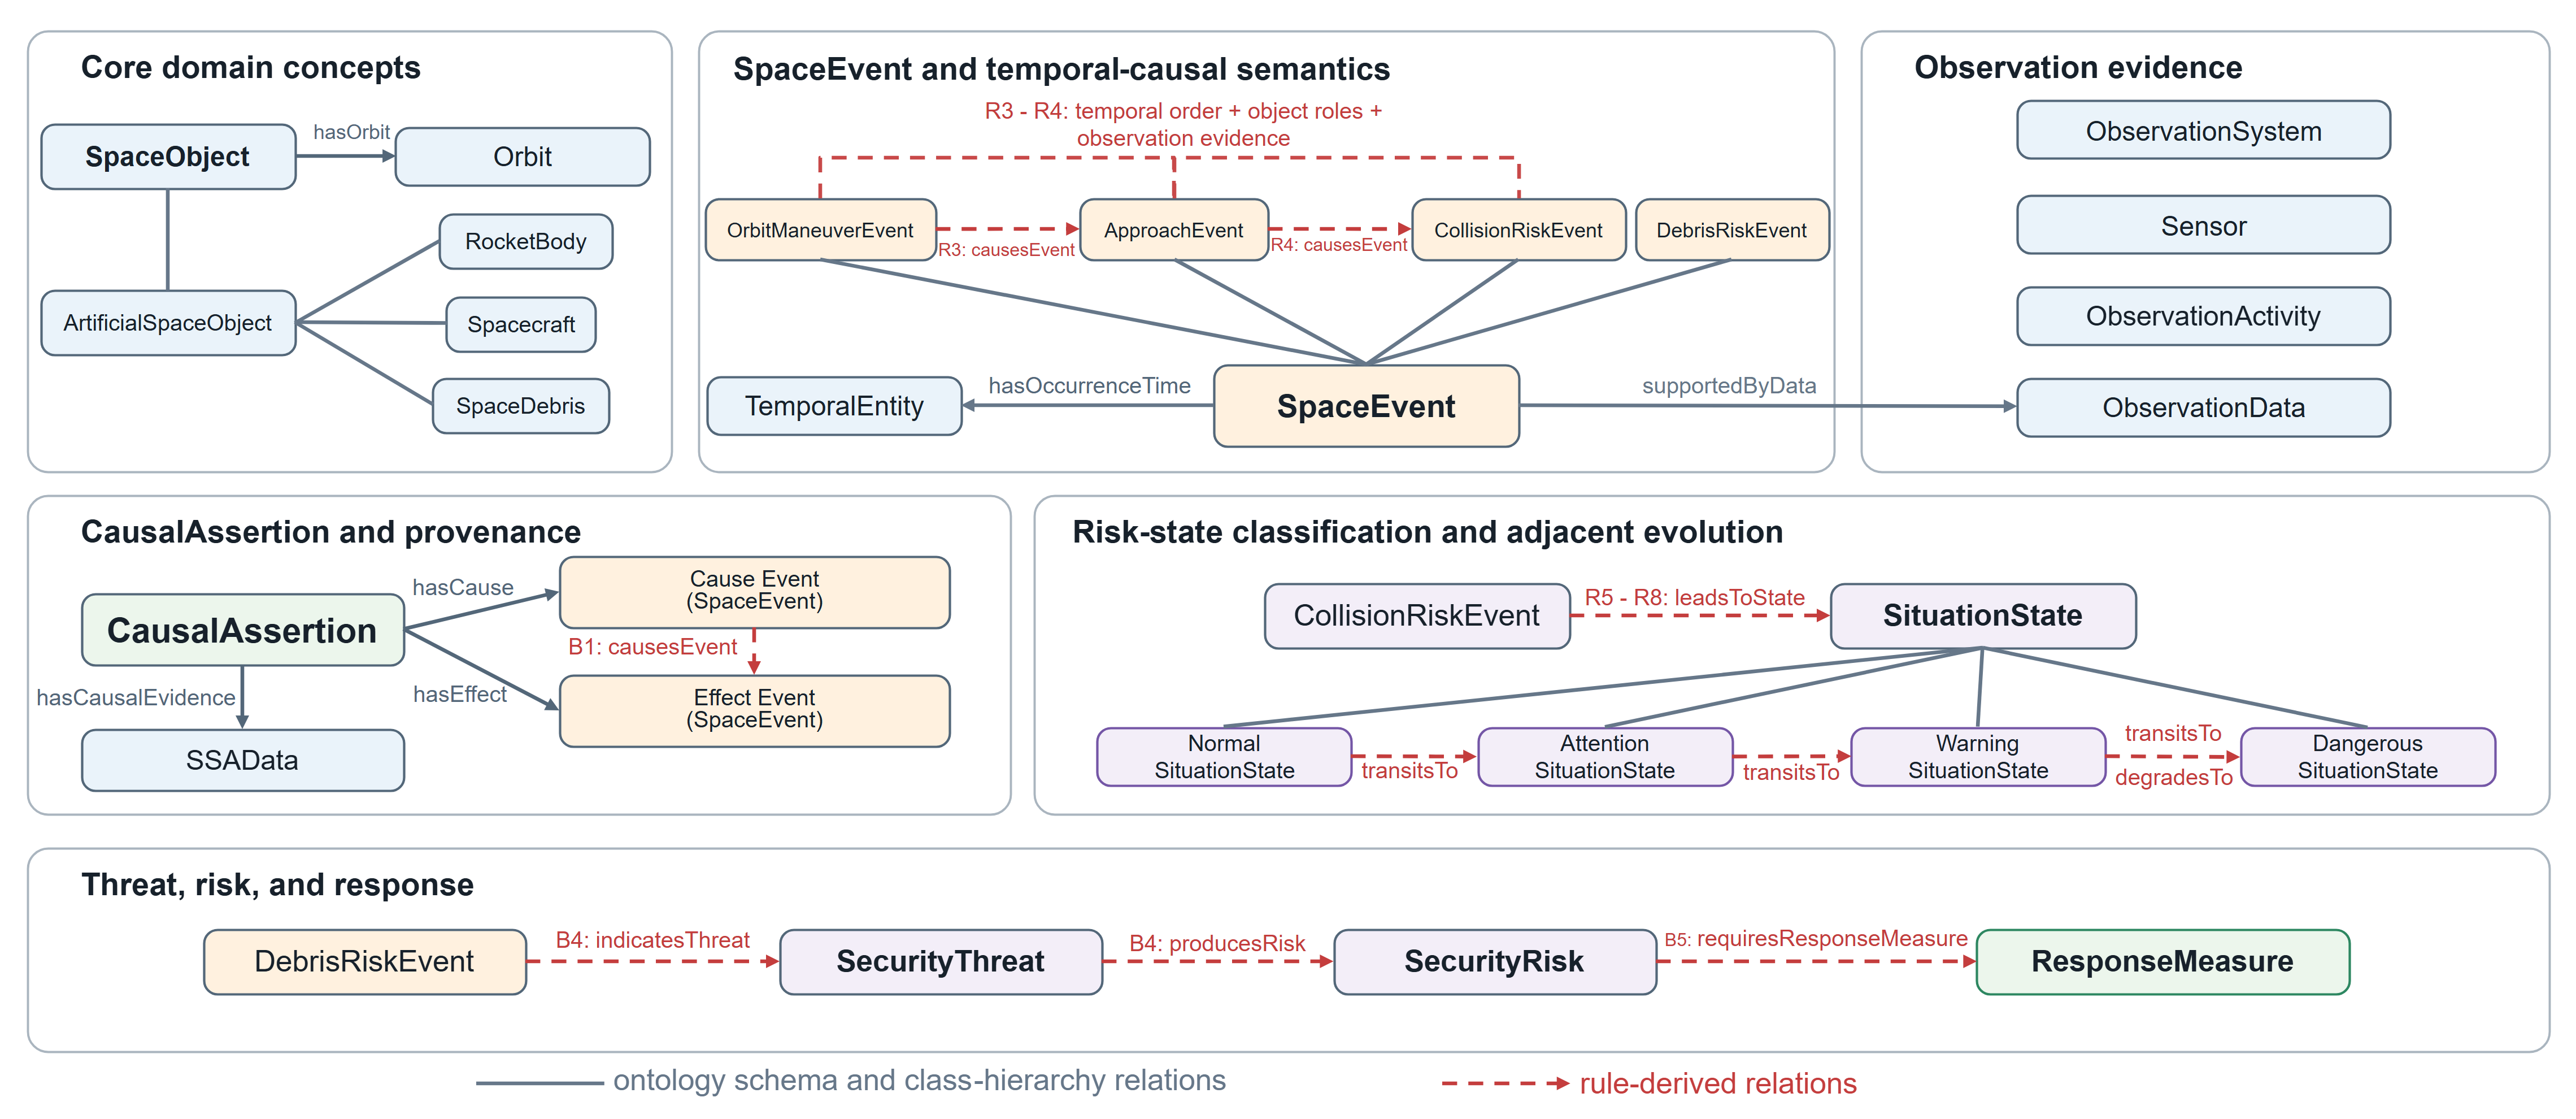
\includegraphics[width=\textwidth]{fig1_core_concepts.png}
  \caption{Core concepts and semantic relations in TC-SSSAO. Solid arrows denote ontology-schema and class-hierarchy relations, and red dashed arrows denote rule-derived relations.}
  \label{fig:core-concepts}
\end{figure}

Figure~\ref{fig:core-concepts} presents the overall semantic framework of TC-SSSAO. \ont{SpaceEvent} serves as the core of knowledge organization. Space objects, orbital information, and observation data provide the basic facts for event representation. Temporal relations describe the order and overlap of events. Event types, object roles, temporal conditions, and observation evidence further support the derivation of directional event relations. Risk parameters are mapped to situation states, and state relations represent changes between adjacent assessments. Security risks and response measures extend the event representation to space-security decision knowledge. Accordingly, TC-SSSAO organizes knowledge through the process \ont{SpaceObject}/Observation $\rightarrow$ \ont{SpaceEvent} $\rightarrow$ Temporal Relations/Event Relations $\rightarrow$ \ont{SituationState} $\rightarrow$ Response.

\subsection{Modeling requirements}

The three requirements identified in Section 1 guide the design of TC-SSSAO. Within the framework shown in Figure~\ref{fig:core-concepts}, they define the modeling requirements for event-centered representation, evidence-constrained event associations, and risk-state evolution.

Firstly, event-centered representation requires explicit connections among space events, participating objects, orbital information, observation data, and temporal information. \ont{SpaceEvent} serves as the organizing core. The model must preserve event identity, participant roles, and supporting data. These connections provide the temporal and evidential context for each event.

Secondly, evidence-constrained event reasoning requires distinct representations of temporal relations and directional event associations. Temporal relations describe event order and overlap. Directional associations depend on event types, object roles, temporal conditions, and observation evidence. The model must retain the supporting evidence and association context to enable traceability of the derived relationships.

Thirdly, risk-state evolution requires explicit assessment-specific states and relationships between adjacent assessments. Each assessment must retain its conjunction encounter identifier, primary and secondary objects, and assessment time. Adjacency is determined within the same encounter and primary-secondary object pair. Adjacent assessments must have strictly ordered times and no intervening assessment within that encounter and object pair. The model must support relationships for increases and decreases in risk severity.

These requirements guide the concepts and properties, risk-state model, reasoning rules, and consistency constraints presented in the following sections.

\subsection{Core concepts and property modeling}
\label{sec:modeling}

\subsubsection{Basic facts and space events}

TC-SSSAO represents space objects with \ont{SpaceObject} and links them to orbital knowledge through \ont{hasOrbit}. \ont{ArtificialSpaceObject} includes \ont{Spacecraft}, \ont{RocketBody}, and \ont{SpaceDebris}. The observation layer is organized around \ont{ObservationSystem} and \ont{Sensor}. Observation activities and their data are represented by \ont{ObservationActivity}, \ont{ObservationData}, and other \ont{SSAData}. Relations including \ont{detectedFromData} and \ont{supportedByData} connect events with observation or assessment data and preserve their data provenance.

The event layer uses \ont{SpaceEvent} as its upper-level concept and includes the principal classes \ont{OrbitManeuverEvent}, \ont{ApproachEvent}, \ont{CollisionRiskEvent}, and \ont{DebrisRiskEvent}. In particular, $\ontm{CollisionRiskEvent}\sqsubseteq\ontm{RiskEvent}$ and $\ontm{CollisionRiskEvent}\sqsubseteq\ontm{SpatialRelationEvent}$.
Every collision-risk event requires a conjunction-encounter identifier. An existential restriction on \ont{CollisionRiskEvent} specifies this requirement: $\ontm{CollisionRiskEvent}\sqsubseteq\exists\,\ontm{hasEncounterID}.\,\ontm{xsd:string}$.
\ont{SpaceEvent} instances are connected to space objects through \ont{involvesObject}, \ont{affectsObject}, \ont{hasPrimaryObject}, and \ont{hasSecondaryObject}. Their temporal information is represented by \ont{hasOccurrenceTime}, \ont{hasStartTime}, and \ont{hasEndTime}. This event-centered structure represents the states and activities of a space object as separate events at different times. Each event can then be associated with temporal information, observation evidence, and risk states. Selected instance and class labels use shortened forms, and all class and property mappings use the formal ontology names defined in TC-SSSAO.

The principal properties used for event representation, temporal relations, event associations, and state evolution are summarized in Table~\ref{tab:core-properties}. Their detailed semantics are introduced in the following subsections.

\begin{table}[!t]
  \centering
  \caption{Principal properties of TC-SSSAO.}
  \label{tab:core-properties}
  \footnotesize
  \begin{tabularx}{\textwidth}{YYY}
    \toprule
    \textbf{Property} & \textbf{Domain/Range} & \textbf{Principal semantics} \\
    \midrule
    \ont{hasPrimaryObject}/\ont{hasSecondaryObject} & \ont{SpatialRelationEvent}$\rightarrow$\ont{SpaceObject} & Object roles in a conjunction \\
    \ont{supportedByData} & \ont{SpaceEvent}$\rightarrow$\ont{SSAData} & Event evidence source \\
    \ont{precedesEvent} & \ont{SpaceEvent}$\rightarrow$\ont{SpaceEvent} & Temporal precedence \\
    \ont{overlapsWithEvent} & \ont{SpaceEvent}$\rightarrow$\ont{SpaceEvent} & Interval intersection \\
    \ont{causesEvent} & \ont{SpaceEvent}$\rightarrow$\ont{SpaceEvent} & Directional event association \\
    \ont{hasCausalEvidence} & \ont{CausalAssertion}$\rightarrow$\ont{SSAData} & Evidence retained by an assertion \\
    \ont{leadsToState} & \ont{SpaceEvent}$\rightarrow$\ont{SituationState} & State corresponding to an event \\
    \ont{hasSourceState}/\ont{hasTargetState} & \ont{StateTransition}$\rightarrow$\ont{SituationState} & Transition endpoints \\
    \ont{transitsTo} & \ont{SituationState}$\rightarrow$\ont{SituationState} & General state-transition relation \\
    \ont{degradesTo}/\ont{recoversTo} & \ont{SituationState}$\rightarrow$\ont{SituationState} & Worsening/recovery specializations \\
    \ont{hasSeverityRank} & \ont{SituationState}$\rightarrow$Integer & State severity \\
    \bottomrule
  \end{tabularx}
\end{table}

\subsubsection{Temporal event relations}

Let $t_i^s$ and $t_i^e$ denote the start and end times of event $e_i$. When $t_1^e<t_2^s$,
\begin{equation}
\fitmath{
\ontm{precedesEvent}(e_1,e_2)\land\ontm{followsEvent}(e_2,e_1).
}
\end{equation}
For two events represented by temporal intervals, TC-SSSAO defines the domain-level interval-intersection relation \ont{overlapsWithEvent}. When $t_1^s<t_2^e\land t_2^s<t_1^e$, the rule derives $\ontm{overlapsWithEvent}(e_1,e_2)$.
This condition denotes a temporal intersection of positive duration, excluding intervals that meet only at a boundary. It is inspired by interval-based temporal reasoning but is intentionally broader than Allen's strict \emph{overlaps} relation~\citep{allen1983}. These properties convert time values into explicit event structures for subsequent directional event association and adjacent-state analysis.

\subsubsection{Causal semantics for events}

TC-SSSAO uses \ont{causesEvent} to represent a directional association between two space events. Temporal order alone does not determine this relation. Three groups of conditions are considered. The first group specifies the temporal relation between the events. The second group specifies their event types and space-object roles. The third group specifies the required observation evidence. For an event $e$, $E_{\mathrm{obs}}(e)$ indicates that the required observation evidence is available. For two events $e_i$ and $e_j$, $T(e_i,e_j)$ denotes the temporal condition, and $O(e_i,e_j)$ denotes the required event-type and object-role conditions. The general rule pattern is
\[
\fitmath{
T(e_i,e_j)\land O(e_i,e_j)
\land E_{\mathrm{obs}}(e_i)
\land E_{\mathrm{obs}}(e_j)
\Rightarrow\ontm{causesEvent}(e_i,e_j).
}
\tag{2}
\]
Temporal precedence is required by the directional association rules. However, temporal precedence alone is not sufficient to establish a \ont{causesEvent} relation. Therefore,
\[
\fitmath{
\ontm{precedesEvent}(e_i,e_j)\nRightarrow\ontm{causesEvent}(e_i,e_j).
}
\tag{3}
\]
\setcounter{equation}{3}
A \ont{causesEvent} relation is generated only when the required event-type, object-role, temporal, and observation-evidence conditions are jointly satisfied. Thus, \ont{causesEvent} represents a rule-constrained directional domain association.

For the maneuver-to-approach association, an earlier \ont{OrbitManeuverEvent} must affect the object that later appears as the primary object of an \ont{ApproachEvent}. The temporal and observation-evidence conditions must also be satisfied. This relation represents a domain-specific maneuver-to-approach association under the stated temporal, object-role, and evidence conditions.

For knowledge that must preserve cause, effect, and evidential context explicitly, TC-SSSAO defines \ont{CausalAssertion}:
\begin{equation}
\fitmath{
\begin{gathered}
\ontm{CausalAssertion}\sqsubseteq
(\geq1\,\ontm{hasCause}.\ontm{SpaceEvent})\\
{}\sqcap(=1\,\ontm{hasEffect}.\ontm{SpaceEvent})\\
{}\sqcap(\geq1\,\ontm{hasCausalEvidence}.\ontm{SSAData}).
\end{gathered}
}
\end{equation}
TC-SSSAO represents event associations in two forms. A direct \ont{causesEvent} relation can be derived from event types, temporal direction, space-object roles, and observation evidence. An explicitly represented \ont{CausalAssertion} can also be projected into a direct \ont{causesEvent} relation for querying and subsequent reasoning. The direct edge provides a concise event-to-event relation. When a \ont{CausalAssertion} is explicitly represented, it retains the provenance context associated with the projected direct relation~\citep{lebo2013provo}.

\subsection{Risk-state representation and adjacent-state evolution}

\subsubsection{Four-level risk states}

TC-SSSAO represents risk situations with \ont{SituationState}. Its four formal subclasses are \ont{NormalSituationState}, \ont{AttentionSituationState}, \ont{WarningSituationState}, and \ont{DangerousSituationState}. Their \ont{hasSeverityRank} values are 0, 1, 2, and 3, respectively. Hereafter, the shortened labels \ont{Normal}, \ont{Attention}, \ont{Warning}, and \ont{Dangerous} refer to those four classes.

For a collision-risk event $e$, $P_c$ denotes the collision probability, $d$ denotes the predicted miss distance, and $h(e)$ denotes the combined hard-body radius of the two involved objects. TC-SSSAO uses two probability thresholds. The parameter $\theta_A$ defines the boundary between the Normal and Attention probability regions. The parameter $\theta_M$ defines the high-probability condition used by Warning and Dangerous. The thresholds satisfy $0\leq\theta_A<\theta_M\leq1$.
Two Boolean conditions are defined as $H_p=(P_c>\theta_M)$ and $H_d=(d<h(e))$.
The risk state is
\begin{equation}
\fitmath{
\text{State}(e)=
\begin{cases}
\ontm{Normal}, & P_c\leq\theta_A\land\neg H_d,\\
\ontm{Attention}, & \theta_A<P_c\leq\theta_M\land\neg H_d,\\
\ontm{Warning}, & H_p\oplus H_d,\\
\ontm{Dangerous}, & H_p\land H_d
\end{cases}
,
}
\label{eq:state-def}
\end{equation}
where $\oplus$ denotes exclusive OR (XOR). Warning is assigned when exactly one of $H_p$ and $H_d$ is satisfied. Dangerous is assigned when both conditions are satisfied. The condition $d<h(e)$ indicates that the predicted miss distance is smaller than the combined hard-body radius. If $d<h(e)$ and $P_c\leq\theta_M$, the snapshot is classified as Warning.

NASA Conjunction Assessment Risk Analysis (CARA) operational guidance uses $P_c>10^{-7}$ as an attention-level reference and $P_c>10^{-4}$ as an important collision-risk mitigation threshold~\citep{nasa_cara_risk,nasa_cara_handbook}. TC-SSSAO therefore uses $\theta_M=10^{-4}$ as the high-risk reference and $\theta_A=10^{-7}$ as an ontology-level boundary that subdivides the low-risk range between \ont{Normal} and \ont{Attention}. The resulting four-state partition is used as the TC-SSSAO risk-state semantics. The TraCSS sensitivity experiments further examine how the two probability thresholds affect state assignments.

\subsubsection{Adjacent-state evolution}

\ont{StateTransition} represents a change between two situation states under repeated assessments. \ont{hasSourceState} and \ont{hasTargetState} record the transition endpoints. \ont{triggeredByEvent} records the triggering event. At the schema level, \ont{transitsTo} denotes a general state-transition relation. The properties \ont{degradesTo} and \ont{recoversTo} represent worsening and recovery transitions, respectively. In the current rule implementation, B2 projects explicitly represented \ont{StateTransition} instances into \ont{transitsTo} relations:
\begin{equation}
\fitmath{
\begin{aligned}
&\ontm{StateTransition}(T_{ij})\land\ontm{hasSourceState}(T_{ij},S_i)\\
&\land\ontm{hasTargetState}(T_{ij},S_j)
\Rightarrow\ontm{transitsTo}(S_i,S_j).
\end{aligned}
}
\end{equation}

B3 automatically materializes severity changes between adjacent risk snapshots. Adjacency is defined only within a single conjunction encounter: two snapshots $e_i$ and $e_j$ are adjacent when they carry the same conjunction-event identifier \ont{hasEncounterID} and the same primary-secondary object pair, the actual assessment time of $e_i$ is strictly earlier than that of $e_j$, and no other \ont{CollisionRiskEvent} with the same encounter identifier and object pair has an assessment time strictly between them. This condition is denoted by $\mathrm{adjacent}(e_i,e_j)$ and prevents adjacency from crossing different conjunction encounters. Let $\mathrm{rank}(S)$ denote the \ont{hasSeverityRank} value of state $S$. For rated states with $\mathrm{rank}(S_i)<\mathrm{rank}(S_j)$, B3 derives $\ontm{transitsTo}(S_i,S_j)$.
For a \ont{WarningSituationState}-to-\ont{DangerousSituationState} transition, B3 additionally derives $\ontm{degradesTo}(S_i,S_j)$.
For adjacent rated states with $\mathrm{rank}(S_i)>\mathrm{rank}(S_j)$, B3 automatically derives both \ont{transitsTo} and \ont{recoversTo}, including recovery across multiple severity levels. Equal-severity assessments produce no transition relation. B3 creates direct relations between assessment-specific state instances and does not create \ont{StateTransition} instances. Explicit transition records remain distinct: B2 projects their source and target states into \ont{transitsTo}, while explicitly asserted recovery relations can also be represented through \ont{recoversTo}.

\subsection{Space-security situation reasoning}
\label{sec:reasoning}

Let $G_0$ be the initial knowledge graph and $\Delta G$ the facts generated by rules. The inferred graph is
\begin{equation}
\fitmath{
G^{*}=G_0\cup\Delta G.
}
\end{equation}

The numbered reasoning and consistency rules are summarized in Tables~\ref{tab:rule-division} and~\ref{tab:rule-division-validation}. R1--R8 derive temporal relations, directional event associations, and risk states. B1--B5 provide semantic projection and bridge relations. R9--R18 validate explicit instance-level and semantic conditions through SHACL shapes with SPARQL-based constraints~\citep{shacl2017,sparql2013}. SHACL Advanced Features provides the rule framework for materializing inferred triples~\citep{shaclaf2017}.

\begingroup
\footnotesize
\setlength{\tabcolsep}{3pt}
\begin{longtable}{@{}>{\raggedright\arraybackslash}p{0.06\textwidth}>{\raggedright\arraybackslash}p{0.28\textwidth}>{\raggedright\arraybackslash}p{0.37\textwidth}>{\raggedright\arraybackslash}p{0.20\textwidth}@{}}
\caption{Summary of TC-SSSAO reasoning rules (R1--R8).}\label{tab:rule-division}\\
\toprule
    \textbf{Rule} &
    \textbf{Main condition} &
    \textbf{Generated fact / validation} &
    \textbf{Validation} \\
    \midrule
\endfirsthead
\caption[]{Summary of TC-SSSAO reasoning rules (R1--R8). (continued)}\\
\toprule
    \textbf{Rule} &
    \textbf{Main condition} &
    \textbf{Generated fact / validation} &
    \textbf{Validation} \\
    \midrule
\endhead
\midrule
\multicolumn{4}{r}{Continued on next page}\\
\endfoot
\bottomrule
\endlastfoot


    R1 &
    Event end/start times satisfy $t_1^e<t_2^s$ &
    \ont{precedesEvent}, \ont{followsEvent} &
    CQ2; CF-2; semantic regression \\
    R2 &
    Event temporal intervals intersect &
    \ont{overlapsWithEvent} &
    CQ2; semantic regression \\
    R3 &
    Maneuver--approach role match, temporal precedence, and observation evidence &
    \ont{causesEvent} from maneuver to approach &
    CQ3; CF-1; CF-2; semantic regression \\
    R4 &
    Same conjunction pair, temporal precedence, and observation evidence &
    \ont{causesEvent} from approach to collision-risk event &
    CQ3; CF-1 (control); semantic regression \\
    R5 &
    Evidence, $P_c\leq\theta_A$, and $d\geq h(e)$ &
    \ont{NormalSituationState} and \ont{leadsToState} &
    CQ5; TraCSS batch; semantic regression \\
    R6 &
    Evidence, $\theta_A<P_c\leq\theta_M$, and $d\geq h(e)$ &
    \ont{AttentionSituationState} and \ont{leadsToState} &
    CQ5; TraCSS batch; semantic regression \\
    R7 &
    Evidence and $H_p\oplus H_d$ &
    \ont{WarningSituationState} and \ont{leadsToState} &
    CQ5; TraCSS batch; CF-3; semantic regression \\*
    R8 &
    Evidence and $H_p\land H_d$ &
    \ont{DangerousSituationState} and \ont{leadsToState} &
    CQ5; TraCSS batch; CF-3; semantic regression \\
    
  \end{longtable}
\endgroup

\begingroup
\footnotesize
\setlength{\tabcolsep}{3pt}
\begin{longtable}{@{}>{\raggedright\arraybackslash}p{0.06\textwidth}>{\raggedright\arraybackslash}p{0.28\textwidth}>{\raggedright\arraybackslash}p{0.37\textwidth}>{\raggedright\arraybackslash}p{0.20\textwidth}@{}}
\caption{Summary of TC-SSSAO consistency and bridge rules (R9--R18 and B1--B5).}\label{tab:rule-division-validation}\\
\toprule
    \textbf{Rule} &
    \textbf{Main condition} &
    \textbf{Generated fact / validation} &
    \textbf{Validation} \\
    \midrule
\endfirsthead
\caption[]{Summary of TC-SSSAO consistency and bridge rules (R9--R18 and B1--B5). (continued)}\\
\toprule
    \textbf{Rule} &
    \textbf{Main condition} &
    \textbf{Generated fact / validation} &
    \textbf{Validation} \\
    \midrule
\endhead
\midrule
\multicolumn{4}{r}{Continued on next page}\\
\endfoot
\bottomrule
\endlastfoot

    R9 &
    \ont{causesEvent} conflicts with event-time direction &
    Causal-time violation &
    CF-2 (negative check); semantic regression \\
    R10 &
    Reciprocal \ont{causesEvent} relations between two distinct events &
    Bidirectional-causality violation &
    CF-2 (negative check); semantic regression \\
    R11 &
    A \ont{causesEvent} path returns to its source event &
    Causal-cycle violation &
    CF-2 (negative check); semantic regression \\
    R12 &
    \ont{SecurityThreat} lacks a required response measure &
    Cardinality violation &
    Semantic regression \\
    R13 &
    \ont{SpaceEvent} lacks observation-data evidence &
    Evidence violation &
    CF-1; semantic regression \\
    R14 &
    Situation-state start time is later than its end time &
    Temporal violation &
    Semantic regression \\
    R15 &
    \ont{ResponseMeasure} has no associated space event &
    Cardinality violation &
    Semantic regression \\
    R16 &
    \ont{SpaceObject} lacks an orbit &
    Cardinality violation &
    Semantic regression \\
    R17 &
    \ont{ObservationSystem} generates no observation data &
    Data-generation violation &
    Semantic regression \\
    R18 &
    Environment level lies outside the allowed value set &
    Value violation &
    Semantic regression \\
    B1 &
    \ont{CausalAssertion} has cause and effect events &
    Direct \ont{causesEvent} &
    CQ4; semantic regression \\
    B2 &
    \ont{StateTransition} has source and target states &
    \ont{transitsTo} &
    CQ6; semantic regression \\
    B3 &
    Adjacent snapshots of the same encounter and object pair have different severity &
    \ont{transitsTo}; \ont{degradesTo} (Warning-to-Dangerous); \ont{recoversTo} (severity decrease) &
    CQ6; semantic regression \\
    B4 &
    \ont{DebrisRiskEvent} is supported by \ont{RiskAssessmentData} &
    Threat and risk relations &
    CQ7; semantic regression \\
    B5 &
    A response measure is explicitly linked to a debris-risk event &
    Response relations among events, threats, and risks &
    CQ7; semantic regression \\
    
  \end{longtable}
\endgroup

Tables~\ref{tab:rule-division} and~\ref{tab:rule-division-validation} list the numbered rules implemented in the TC-SSSAO rule layer. Additional numerical and structural input checks are implemented outside R1--R18. These checks include collision-probability ranges, nonnegative distance values, single-valued risk parameters, and primary-secondary object consistency. They serve as input-validation conditions in the experimental pipeline and are therefore not listed as numbered rules in these tables. CQ denotes a competency question, and CF denotes a condition-change or counterfactual experiment. Their implementations are described in Section~\ref{sec:capability-verification}.

Let $M(e)$, $A(e)$, and $C(e)$ denote that event $e$ is an instance of \ont{OrbitManeuverEvent}, \ont{ApproachEvent}, and \ont{CollisionRiskEvent}, respectively. Let $E_{\mathrm{obs}}(e)$ indicate that event $e$ has the required observation evidence. The predicate $\mathrm{samePair}(e_i,e_j)$ indicates that the two events have the same primary and secondary objects. Let $t(e)$ denote the occurrence time of event $e$. For an orbital-maneuver event $e_1$ and an approach event $e_2$, R3 is
\begin{equation}
\fitmath{
\begin{aligned}
&M(e_1)\land A(e_2)\land\ontm{affectsObject}(e_1,o_1)\\
&\land\ontm{hasPrimaryObject}(e_2,o_1)
\land\ontm{hasSecondaryObject}(e_2,o_2)\land o_1\neq o_2\\
&\land\ontm{precedesEvent}(e_1,e_2)
\land E_{\mathrm{obs}}(e_1)\land E_{\mathrm{obs}}(e_2)\\
&\Rightarrow\ontm{causesEvent}(e_1,e_2),
\end{aligned}
}
\end{equation}
where \ont{hasSecondaryObject} identifies the secondary object and $o_1\neq o_2$ specifies distinct primary and secondary objects.

For an approach event $e_1$ and a collision-risk event $e_2$, R4 is
\begin{equation}
\fitmath{
\begin{aligned}
&A(e_1)\land C(e_2)\land\text{samePair}(e_1,e_2)\\
&\land\ontm{precedesEvent}(e_1,e_2)
\land E_{\mathrm{obs}}(e_1)\land E_{\mathrm{obs}}(e_2)\\
&\Rightarrow\ontm{causesEvent}(e_1,e_2).
\end{aligned}
}
\end{equation}

R4 links an approach event to a collision-risk event through \ont{causesEvent}. The two events must share the same primary and secondary objects and satisfy the temporal and evidence conditions.

Under the conditions defined by R3 and R4, the two derived \ont{causesEvent} relations form the following directional association path:
\[
\fitmath{
\ontm{OrbitManeuverEvent}
\rightarrow
\ontm{ApproachEvent}
\rightarrow
\ontm{CollisionRiskEvent}.
}
\]
The first edge represents the maneuver-to-approach association derived by R3. The second edge represents the approach-to-collision-risk association derived by R4. This path exists only when the corresponding temporal, object-role, and observation-evidence conditions are satisfied.


\subsection{Knowledge-consistency constraints}

TC-SSSAO uses R9--R18 to validate explicit instance-level and semantic conditions. R9 checks consistency between directional event relations and event time. R10 detects reciprocal \ont{causesEvent} relations between distinct events, and R11 detects causal cycles. R12--R18 further check required response knowledge, event evidence, state-time consistency, response-event association, object-orbit association, observation-data generation, and environment-level values. Violations are reported through SHACL validation~\citep{shacl2017}.

Additional input conditions are checked at the implementation level during experimental processing. These conditions include valid collision-probability ranges, nonnegative distance values, single-valued risk parameters, and consistency between primary and secondary objects. They complement the numbered SHACL constraints but are not part of R9--R18.

For example, when
\begin{equation}
\fitmath{
\ontm{causesEvent}(e_1,e_2)\land t(e_1)>t(e_2),
}
\tag{10}
\end{equation}
\setcounter{equation}{10}
R9 reports a conflict between the directional event relation and temporal order. SHACL validation reports preserve the affected instances and the corresponding constraint information.
\section{Experimental Validation}

This chapter validates the three modeling requirements defined in Sections 1 and 3.1: event-centered knowledge representation, evidence-constrained event associations, and risk-state evolution. Ontology quality validation establishes the structural and logical basis for the experiments. Seven competency questions (CQ1--CQ7) examine evidence retrieval, event relations, risk states, state transitions, and response knowledge. Counterfactual experiments test the observation-evidence and temporal conditions of directional event reasoning. The TraCSS experiments examine the four risk-state conditions and threshold sensitivity across a large conjunction dataset. The CZ-6A case connects real-event facts, evidence, event relations, and response knowledge within the ontology.

\subsection{Data and experimental design}
\label{sec:experimental-design}

The experiments use three types of input: controlled rule scenarios, TraCSS conjunction records, and CZ-6A case knowledge. The controlled scenarios test individual rules and adjacent-state evolution. TraCSS records support large-scale risk-state classification and threshold analysis. The CZ-6A case supports event-centered knowledge instantiation and integrated reasoning. The following subsections describe the two empirical sources, the experimental design, and the construction of the controlled scenarios.

\subsubsection{TraCSS data}
\label{sec:tracss-data}

The TraCSS risk-state experiment uses the Conjunction Assessment Verification Dataset released by the Office of Space Commerce~\citep{tracss_dataset}. The experiment uses the discrete hard-body-radius (HBR) results and the object-level HBR mapping file described in the accompanying user's guide~\citep{tracss_users_guide}. The raw data contain 283,595 conjunction records. Among them, 38 records have missing collision probabilities. After excluding the 38 records with missing collision probabilities, 283,557 valid records remain for analysis.

The selected fields connect the dataset to the event and risk representations defined in Section 3. They include conjunction ID, object 1, object 2, time of closest approach (TCA), collision probability, minimum range, and object HBR. In TraCSS, the \texttt{prob} field reports collision probability on a linear scale and supplies $P_c$. The \texttt{min\_range} field supplies the predicted miss distance in kilometers, so $d=\texttt{min\_range}$. Object-level HBR values are radii in meters. The combined hard-body radius is converted to kilometers as
\begin{equation}
\fitmath{
h(e)=\frac{\mathrm{HBR}_1+\mathrm{HBR}_2}{1000}\ \mathrm{km}.
}
\end{equation}
The HBR mapping covers the objects in all 283,595 records. Each TraCSS record represents an independent conjunction assessment result. The experiments apply the R5--R8 state-assignment conditions to these records. The controlled scenarios described below provide the successive assessments for testing adjacent-state evolution.

\subsubsection{CZ-6A event data}
\label{sec:cz6a-data}

The CZ-6A case provides the real-event context for the event-centered and evidence-traceability requirements. It represents the Chang Zheng 6A (CZ-6A) 2022-151B upper-stage fragmentation event. NASA orbital-debris material provides the fragmentation and tracking facts~\citep{nasa_odqn}. Wacker et al.~\citep{wacker2025cz6a} provide the source analysis for the debris environment and long-term collision risk. The case knowledge includes the CZ-6A upper stage, orbital information, a fragmentation event, a debris-tracking event, a debris-risk event, observation data, risk-assessment data, a \ont{CausalAssertion}, and a continuous-tracking measure. The source-grounded facts are instantiated with their provenance retained. The continuous-tracking measure supplies application knowledge for the response relations described in Section 3.

\subsubsection{Experimental design}

The three types of input support four validation components. Firstly, ontology quality validation checks build consistency, logical consistency, class satisfiability, modeling practice, and SHACL constraints. Alignment non-regression uses a controlled ontology $C = T - F$. Here, $T$ denotes the aligned ontology, and $F$ contains 16 cross-standard alignment triples. Five checks (A1--A5) examine the effects of the alignment.

Secondly, ontology capability and counterfactual validation examines the three modeling requirements through CQ1--CQ7. CQ1 and CQ7 address evidence and response knowledge within the event-centered structure. CQ2--CQ4 address temporal relations, directional associations, and causal-assertion projection. CQ5 and CQ6 address risk-state generation and state-transition relations. SPARQL queries and controlled rule scenarios implement these questions. Observation-evidence removal and event-time reversal test the event-association conditions. A risk-threshold change tests the boundary between Warning and Dangerous.

Thirdly, the TraCSS risk-state experiments apply a batch implementation of the R5--R8 conditions to the conjunction records. They examine state distributions, partition coverage, and sensitivity to the two probability thresholds. Fourthly, the CZ-6A real-event experiment applies fixed-point reasoning to the case knowledge. It examines the connections among event facts, temporal relations, evidence, threats, risks, and responses. A semantic capability comparison then relates these results to the knowledge models reviewed in Section 2.

\subsubsection{Controlled scenario construction}

{\emergencystretch=1.5em
The controlled scenarios introduced above provide the inputs for the rule and counterfactual experiments. The principal scenario contains 15 explicitly instantiated entities and 120 asserted triples. These entities comprise two space objects, two orbits, one observation system, three data instances, and seven space events. The seven event instances comprise one orbital-maneuver event, one approach event, and five collision-risk assessment snapshots. They instantiate the event classes introduced in Section 3.2.1.

The asserted facts specify event types, object roles, observation evidence, temporal values, encounter identifiers, and risk parameters. The initial graph contains no explicit \ont{precedesEvent}, \ont{causesEvent}, \ont{leadsToState}, \ont{transitsTo}, \ont{degradesTo}, or \ont{recoversTo} relation. It also contains no \ont{SituationState} or \ont{StateTransition} instance. The subsequent reasoning results therefore record the relations and states generated from these input facts.

The scenario connects the input facts to the rule groups described in Section 3. R1 derives temporal precedence. R3 and R4 derive the maneuver--approach--collision-risk directional event-association path. The five collision-risk snapshots use parameter settings for the sequence \ont{Normal}, \ont{Attention}, \ont{Warning}, \ont{Dangerous}, and \ont{Normal}. R5--R8 generate the corresponding assessment-specific states. The final snapshot returns to the Normal level and produces a separate state instance. The five snapshots thus instantiate four state classes across five successive assessments.

All five snapshots share one encounter identifier and primary-secondary object pair. Their assessment times are strictly ordered. B3 materializes the three adjacent increases in severity and the subsequent Dangerous-to-Normal recovery. Separate test graphs exercise B1 causal-assertion projection, B2 explicit-transition projection, and R2 interval intersection.

The counterfactual scenarios modify selected conditions in the principal scenario. CF-1 removes the observation-evidence triple required by R3. CF-2 reverses the temporal order of the target events. Their event types, object roles, evidence links, and durations remain unchanged in CF-2. Each intervention is compared with the original input graph before reasoning. Additional test graphs cover positive and negative boundary conditions for R3--R8, B2, and B3. The SHACL positive graph conforms to the constraint set. The negative graph contains the intended constraint violations.\par}

\subsection{Ontology quality validation}

The first validation component examines the ontology structure, logic, constraints, and rules defined in Section 3. RDF (Resource Description Framework) graph isomorphism~\citep{rdf2014} compares the ontology reconstructed from the authoring sources with the canonical OWL artifact. The HermiT reasoner~\citep{glimm2014hermit} checks logical consistency and class satisfiability. Modeling-practice checks examine domain and range declarations, disjoint and inverse axioms, datatype ranges, class--instance distinctions, and naming and annotation completeness. Positive and negative SHACL graphs test the consistency constraints introduced in Section 3.5. Semantic-regression tests examine the derivation and consistency behavior of R1--R18 and B1--B5.

Table~\ref{tab:ontology-quality} summarizes the validation results. Counts are reported both for the complete canonical graph and for entities defined in the TC-SSSAO namespace so that the counting scope is explicit.

\begin{table}[!t]
  \centering
  \caption{Ontology-quality validation results for TC-SSSAO.}
  \label{tab:ontology-quality}
  \footnotesize
  \begin{tabularx}{\textwidth}{p{0.16\textwidth}p{0.27\textwidth}Y}
    \toprule
    \textbf{Validation item} & \textbf{Method} & \textbf{Result} \\
    \midrule
    Ontology size & Count explicit declarations and triples & 96 named classes in total (86 in the TC-SSSAO namespace); 70 object properties in total (65 in the namespace); 68 data properties in total (68 in the namespace); 17 annotation properties in total (12 in the namespace); 1,703 triples \\
    Axiom inventory & OWLAPI~5 metrics on the canonical ontology~\citep{horridge2011owlapi} & 1,326 OWL axioms in total, including 486 logical axioms, 252 declaration axioms, and 588 annotation assertions \\
    Rule inventory & Count numbered reasoning and consistency rules & 23 numbered rules in total: R1--R18 and B1--B5 \\
    SHACL inventory & Count shapes in the main rule file and auxiliary validation files & 31 NodeShapes in the main rule file, including the 23 numbered rules; 10 additional unnumbered shapes are defined in auxiliary validation files \\
    Build consistency & RDF graph-isomorphism comparison & Rebuilt and canonical ontology graphs both contain 1,703 triples; the isomorphism check passes \\
    Logical consistency & HermiT consistency checking & The ontology is consistent \\
    Class satisfiability & HermiT classification & Zero unsatisfiable classes \\
    Modeling practice & Static checks for missing domain/range, inverse and disjoint declarations, class--instance confusion, datatype-range misuse, and related schema pitfalls & No Critical or Important issues \\
    Constraint validity & Positive and negative SHACL test graphs & The positive graph conforms; the negative graph produces 27 expected violations \\
    Rule semantics & Semantic regression for R1--R18 and B1--B5 & All 58 checks produce the expected results \\
    \bottomrule
  \end{tabularx}
\end{table}

The reconstructed ontology graph is isomorphic to the canonical OWL artifact. The canonical ontology contains 1,326 OWL axioms according to OWLAPI 5. These comprise 486 logical axioms, 252 declaration axioms, and 588 annotation assertions. HermiT reports no inconsistency and no unsatisfiable class. The modeling-practice checks report no Critical or Important issues in the examined categories. The positive SHACL graph conforms to the constraints. The negative graph produces 27 expected violations. The semantic-regression suite contains 58 checks covering R1--R18 and B1--B5. All checks produce the expected results.

All five alignment non-regression checks (A1--A5) pass. Removing the 16 cross-standard alignment triples from $T$ yields a graph isomorphic to $C$. The difference between $T$ and $C$ is exactly $F$. The core relation definitions, entity declarations, and anonymous class structures are preserved. These results establish the structural and semantic basis for testing the three modeling requirements through competency questions and counterfactual experiments.

\subsection{Ontology capability and counterfactual validation}
\label{sec:capability-verification}

Following ontology quality validation, the second component examines the three modeling requirements through the scenarios defined in Section~\ref{sec:experimental-design}. Competency questions test evidence retrieval, event relations, risk-state generation, adjacent-state evolution, and response knowledge. Counterfactual experiments then change observation evidence, temporal direction, and a risk threshold to examine their effects on the derived results.

\subsubsection{Competency question validation}

The seven competency questions connect the modeling requirements to specific queries and rule scenarios. CQ1 retrieves event-linked evidence and addresses the event-centered representation requirement. CQ2 tests R1/R2 temporal relations. A representative SPARQL query~\citep{sparql2013} retrieves the precedence relation derived by R1. CQ3 tests the R3/R4 directional event-association path. CQ4 tests B1 projection from an explicit causal assertion. CQ2--CQ4 thus examine the event-relation mechanisms defined in Sections 3.2 and 3.4.

CQ5 tests four-level risk-state generation through R5--R8. CQ6 tests B2 explicit-transition projection and B3 adjacent-state relations. A SPARQL query retrieves the B3 relations from the post-reasoning graph. These two questions address the risk-state and state-evolution requirement defined in Section 3.3. CQ7 retrieves the threat, risk, and response knowledge connected by B4 and B5 in the fixed-point CZ-6A graph. It extends the event-centered representation to response knowledge. Table~\ref{tab:cq-verification} summarizes the questions, implementations, and outcomes. The following table reports the CQ6 query results.

\begin{table}[!t]
  \centering
  \caption{Competency-question validation results for TC-SSSAO.}
  \label{tab:cq-verification}
  \footnotesize
  \begin{tabularx}{\textwidth}{p{0.05\textwidth}>{\raggedright\arraybackslash}Y>{\raggedright\arraybackslash}Y>{\raggedright\arraybackslash}Y}
    \toprule
    \textbf{CQ} & \textbf{Competency question} & \textbf{Implementation} & \textbf{Result} \\
    \midrule
    CQ1 & Retrieve event evidence & SPARQL query & Returns event-linked observation/assessment data \\
    CQ2 & Retrieve temporal relations & R1/R2 probes; representative SPARQL query for R1 & Derives precedence and inverse relations; R2 separately validates interval intersection \\
    CQ3 & Construct a directional event-association path & R3/R4 controlled rule scenario & Produces the maneuver--approach--collision-risk directional event-association path \\
    CQ4 & Project a causal assertion & B1 rule probe & Generates direct \ont{causesEvent} \\
    CQ5 & Generate risk states & R5--R8 controlled rule scenario & Generates four-level states \\
    CQ6 & Retrieve adjacent-state relations & B2 rule probe; B3 rule scenario + SPARQL query & Returns materialized \ont{transitsTo}, \ont{degradesTo}, and \ont{recoversTo} relations \\
    CQ7 & Query risk response & B4/B5 + SPARQL query & Returns derived threat/risk knowledge linked to the response measure \\
    \bottomrule
  \end{tabularx}
\end{table}

CQ6 uses the five successive assessments introduced in the controlled scenario. The SPARQL query selects source states, relation types, and target states from the post-reasoning graph. It retrieves \ont{transitsTo}, \ont{degradesTo}, and \ont{recoversTo}. The corresponding input graph contains none of these relations. The query returns six bindings: four \ont{transitsTo} relations, one \ont{degradesTo} relation, and one \ont{recoversTo} relation.

The first three \ont{transitsTo} relations form the sequence Normal $\rightarrow$ Attention $\rightarrow$ Warning $\rightarrow$ Dangerous. The Warning-to-Dangerous change also produces \ont{degradesTo}. The fifth assessment generates a distinct Normal state. The Dangerous-to-Normal change produces the fourth \ont{transitsTo} relation and the \ont{recoversTo} relation. B3 materializes all six bindings from the encounter, object-role, time, and severity conditions defined in Section 3.3.2. B2 projection is tested separately with explicit \ont{StateTransition} instances. Table~\ref{tab:cq6-results} lists the returned relations. The state labels identify the classes of the assessment-specific state instances.

\begin{table}[!htbp]
  \centering
  \caption{Returned bindings of the CQ6 state-transition query on the post-reasoning graph.}
  \label{tab:cq6-results}
  \footnotesize
  \begin{tabular}{lll}
    \toprule
    \textbf{Source state} & \textbf{Relation} & \textbf{Target state} \\
    \midrule
    Normal & \ont{transitsTo} & Attention \\
    Attention & \ont{transitsTo} & Warning \\
    Warning & \ont{transitsTo} & Dangerous \\
    Warning & \ont{degradesTo} & Dangerous \\
    Dangerous & \ont{transitsTo} & Normal \\
    Dangerous & \ont{recoversTo} & Normal \\
    \bottomrule
  \end{tabular}
\end{table}
The CQ6 results connect the assessment-specific states through explicit transition relations. CQ7 extends the event-centered structure to threat, risk, and response knowledge. Its SPARQL query follows \ont{indicatesThreat} from the CZ-6A debris-risk event and retrieves the response measure through \ont{requiresResponseMeasure}. It also retrieves the linked risk through \ont{producesRisk} and \ont{mitigatesRisk}. The query returns a derived physical-threat node, a derived debris-risk node, and the explicit \ont{ContinuousTrackingMeasure}. B4 and B5 introduce the threat and risk nodes and their event and response relations. Section~\ref{sec:cz6a-case} presents the complete case reasoning process.

\subsubsection{Observation-evidence condition experiment}

CQ3 establishes the directional event-association path under the original input conditions. CF-1 then tests the observation-evidence requirement of R3. It removes the asserted triple linking \ont{Evt\_Maneuver} to its observation data. Event types, temporal values, object roles, target-event evidence, and all five risk snapshots remain unchanged. R3 derives \ont{causesEvent} in the original scenario. After evidence removal, reasoning from the modified input no longer derives this relation. Table~\ref{tab:evidence-condition} compares the two results.
\begin{table}[!htbp]
  \centering
  \caption{Observation-evidence condition experiment.}
  \label{tab:evidence-condition}
  \footnotesize
  \begin{tabular}{lll}
    \toprule
    \textbf{Condition} & \textbf{Original scenario} & \textbf{After evidence removal} \\
    \midrule
    Temporal condition & Satisfied & Satisfied \\
    Object-role condition & Satisfied & Satisfied \\
    Observation evidence & Present & Absent \\
    \ont{causesEvent} & Derived & Not derived \\
    \bottomrule
  \end{tabular}
\end{table}
The R4 relation retains its original result. R13 reports the missing-evidence violation. These results connect R3 event-association reasoning with the evidence requirement and the R13 consistency constraint described in Section 3. The next experiment examines the temporal condition of the same association.

\subsubsection{Temporal-direction condition experiment}

CF-2 tests the temporal-direction requirement of R3. It replaces the six occurrence/start/end-time triples of the two target events and reverses their temporal order. Their event types, object roles, observation evidence, and durations remain unchanged. In the original scenario, $\ontm{precedesEvent}(\ontm{Evt\_Maneuver},\ontm{Evt\_Approach})$ holds. R3 derives \ont{causesEvent} in the same direction. After the change, R1 derives the reversed \ont{precedesEvent}/\ont{followsEvent} pair. The original precedence relation and the original \ont{causesEvent} relation are absent from the new reasoning result. The reversed temporal relation produces no reversed \ont{causesEvent} relation. R3 retains its event-type and object-role requirements. The experiment produces no bidirectional relation, causal cycle, or causal-time conflict. CF-1 and CF-2 thus demonstrate the joint roles of evidence, time, event type, and object roles in directional event reasoning.

\subsubsection{Risk-state boundary experiment}

Following the event-association experiments, CF-3 examines the risk-state boundary defined in Section 3.3.1. It uses the single TraCSS record satisfying $d<h(e)$: $P_c=6.593401\times10^{-6}$, $d=0.008684$\,km, and $h(e)=0.011017$\,km. At $\theta_M=10^{-4}$, the record satisfies $P_c\leq\theta_M$. R7 therefore assigns Warning. Reducing $\theta_M$ to $10^{-6}$ satisfies both the high-probability and close-range conditions. R8 then assigns Dangerous to the same record. Table~\ref{tab:condition-change} summarizes the evidence, temporal-direction, and risk-boundary experiments.
\begin{table}[!t]
  \centering
  \caption{Summary of condition-change experiments.}
  \label{tab:condition-change}
  \footnotesize
  \begin{tabularx}{\textwidth}{lYYYY}
    \toprule
    \textbf{Experiment} & \textbf{Changed condition} & \textbf{Held constant} & \textbf{Original result} & \textbf{Adjusted result} \\
    \midrule
    CF-1 & Remove observation evidence & Time and roles & \ont{causesEvent} & Not derived \\
    CF-2 & Reverse event time & Types, roles, evidence & Original direction & Not derived \\
    CF-3 & $\theta_M\colon10^{-4}\rightarrow10^{-6}$ & Same TraCSS record & \ont{Warning} & \ont{Dangerous} \\
    \bottomrule
  \end{tabularx}
\end{table}
The three experiments connect changes in input conditions to changes in rule results. CF-1 and CF-2 address evidence-constrained event associations. CF-3 addresses the distinction between Warning and Dangerous. The following section extends this risk-state analysis from one boundary record to the complete TraCSS dataset.

\subsection{TraCSS risk-state experiments}
\label{sec:tracss-experiments}

The third validation component examines the four-level risk-state model across the TraCSS records introduced in Section~\ref{sec:tracss-data}. It first applies the baseline thresholds and examines the underlying probability and distance conditions. Separate and joint threshold scans then characterize changes in state assignments. The controlled CQ6 scenario provides the complementary test of state evolution across successive assessments.

\subsubsection{Baseline state distribution}

The batch implementation applies the R5--R8 state-assignment conditions to the 283,557 valid TraCSS records. It uses the thresholds defined in Section 3.3.1: $\theta_A=10^{-7}$ and $\theta_M=10^{-4}$. The controlled RDF scenarios test the corresponding SHACL-SPARQL rules. Table~\ref{tab:tracss-state-distribution} reports the resulting state distribution across the full dataset.
\begin{table}[!htbp]
  \centering
  \caption{Risk-state distribution on the TraCSS dataset.}
  \label{tab:tracss-state-distribution}
  \footnotesize
  \begin{tabular}{lrr}
    \toprule
    \textbf{Risk state} & \textbf{Count} & \textbf{Percentage} \\
    \midrule
    Normal & 86,585 & 30.54\% \\
    Attention & 196,666 & 69.36\% \\
    Warning & 306 & 0.11\% \\
    Dangerous & 0 & 0.00\% \\
    Total & 283,557 & 100.00\% \\
    \bottomrule
  \end{tabular}
\end{table}
Coverage checks give \texttt{no\_state}=0, \texttt{multi\_state}=0, \texttt{overlap}=0, and \texttt{gap}=0. Every valid record receives exactly one risk state under the baseline parameters. The resulting partition implements the four conditions defined in Section 3.3.1. The baseline Dangerous count is zero. The following condition analysis explains this distribution through the collision-probability and miss-distance values.

\subsubsection{Distribution of risk conditions}

The baseline distribution follows from the two Boolean conditions $H_p$ and $H_d$ defined in Section 3.3.1. Among the valid records, 305 satisfy $P_c>10^{-4}$ and one satisfies $d<h(e)$. These conditions occur in separate records. No baseline record satisfies $P_c>10^{-4}\land d<h(e)$, and the Dangerous count is therefore zero. The close-range record has $d=8.684$\,m, $h(e)=11.017$\,m, and $P_c=6.593401\times10^{-6}$. R7 assigns it to Warning, as reported in CF-3. The 306 Warning records comprise 305 records satisfying $P_c>\theta_M\land d\geq h(e)$ and one satisfying $P_c\leq\theta_M\land d<h(e)$. These groups correspond to the two branches of the exclusive-OR Warning condition. The threshold experiments below examine how changes in $\theta_A$ and $\theta_M$ redistribute these state assignments.

\subsubsection[Theta-A sensitivity]{Sensitivity to $\theta_A$}

The first sensitivity experiment examines the Normal--Attention boundary controlled by $\theta_A$. It fixes $\theta_M=10^{-4}$ and scans $\theta_A$ over $\{10^{-9},10^{-8},10^{-7},10^{-6},10^{-5}\}$. State changes occur between Normal and Attention. Warning remains 306, and Dangerous remains zero. Relative to the baseline, one-order-of-magnitude perturbations reassign approximately 5.36\% and 11.46\% of records. The maximum reassignment within two orders of magnitude is 55.09\%. State counts change monotonically with $\theta_A$. These results connect $\theta_A$ to the low-risk subdivision defined in Section 3.3.1.

\subsubsection[Theta-M sensitivity]{Sensitivity to $\theta_M$}

The second sensitivity experiment examines the high-probability condition controlled by $\theta_M$. It fixes $\theta_A=10^{-7}$ and scans $\theta_M$ over $\{10^{-6},10^{-5},10^{-4},10^{-3},10^{-2}\}$. Table~\ref{tab:theta-m-sensitivity} reports the results. The Warning counts are 164,485, 40,766, 306, 1, and 1, respectively. At $\theta_M=10^{-6}$, the close-range record also satisfies $P_c>\theta_M$. R8 assigns it to Dangerous. This result reproduces the boundary behavior described in CF-3 within the full-dataset experiment.
\begin{table}[!htbp]
  \centering
  \caption{Sensitivity results for $\theta_M$.}
  \label{tab:theta-m-sensitivity}
  \footnotesize
  \begin{tabular}{lrr}
    \toprule
    $\theta_M$ & \textbf{Warning} & \textbf{Dangerous} \\
    \midrule
    $10^{-6}$ & 164,485 & 1 \\
    $10^{-5}$ & 40,766 & 0 \\
    $10^{-4}$ & 306 & 0 \\
    $10^{-3}$ & 1 & 0 \\
    $10^{-2}$ & 1 & 0 \\
    \bottomrule
  \end{tabular}
\end{table}
For the close-range record with $P_c=6.593401\times10^{-6}$, the boundary is $\theta_M<P_c\Rightarrow\ontm{Dangerous}$ and $\theta_M\geq P_c\Rightarrow\ontm{Warning}$.

\subsubsection{Joint sensitivity}

The separate scans identify the roles of the two thresholds. A further $3\times3$ scan examines their combined effects. It combines $\theta_A\in\{10^{-8},10^{-7},10^{-6}\}$ with $\theta_M\in\{10^{-5},10^{-4},10^{-3}\}$. Normal varies mainly with $\theta_A$. Warning varies mainly with $\theta_M$. Dangerous remains zero in all nine combinations, and no additional state-assignment conflicts occur. Across all scanned parameters and diagnostic points, the experiments produce no unclassified record, multiple assignment, condition overlap, or condition gap. Complete partition coverage is preserved. The baseline parameters remain $\theta_A=10^{-7}$ and $\theta_M=10^{-4}$.

The TraCSS results characterize the numerical state-assignment component of the risk-state requirement. CQ6 demonstrates the corresponding relations between successive assessment-specific states. The next experiment returns to the event-centered representation requirement and applies the ontology to real-event knowledge.

\subsection{Real-event case: CZ-6A}
\label{sec:cz6a-case}

The fourth validation component connects the individual mechanisms tested above within a real-event knowledge graph. The CZ-6A case uses the event, observation, and provenance structure introduced in Section 3.2. Temporal reasoning and the B1, B4, and B5 bridge rules connect the case facts to event associations, threats, risks, and response knowledge.

\subsubsection{Case knowledge base}

The source material described in Section~\ref{sec:cz6a-data} is instantiated as an initial knowledge graph containing 136 case triples. The graph links the upper stage, orbital information, fragmentation, tracking, and debris-risk events to their supporting data. The experiment loads the canonical TC-SSSAO ontology, the case instances, and the SHACL-SPARQL rules. It combines OWL/RDFS reasoning~\citep{owl2,rdfs2014} with SHACL-SPARQL fixed-point reasoning~\citep{shacl2017,shaclaf2017}.

The initial graph contains the debris-risk event and its explicit \ont{CausalAssertion}. The continuous-tracking measure supplies application knowledge for the response relations. During reasoning, B1 projects the assertion into a direct \ont{causesEvent} relation. B4 derives threat and risk knowledge from the debris-risk event. B5 connects the response measure to this knowledge. This sequence applies the assertion-projection and response mechanisms described in Section 3 and tested through CQ4 and CQ7.

\subsubsection{Case results}

The CZ-6A case reaches a fixed point after three iterations. The case graph grows from 136 to 367 triples, adding 231 statements. The graph conforms to the SHACL constraints. Table~\ref{tab:cz6a-results} groups the results by temporal relations, event associations, threat and risk knowledge, response relations, and evidence traceability. These categories follow the event-centered knowledge structure defined in Section 3.
\begin{table}[!t]
  \centering
  \caption{Experimental results for the CZ-6A real-event case.}
  \label{tab:cz6a-results}
  \footnotesize
  \begin{tabularx}{\textwidth}{lY}
    \toprule
    \textbf{Validation item} & \textbf{Reasoning result} \\
    \midrule
    Event time & Derives the temporal relation from fragmentation to subsequent tracking \\
    Event association & B1 projects the explicit fragmentation--debris-risk \ont{CausalAssertion} into \ont{causesEvent} \\
    Threat and risk & Connects the debris-risk event with a derived physical threat and debris risk \\
    Response measure & Connects the explicit continuous-tracking measure with the event, threat, and risk \\
    Evidence traceability & Returns the NASA tracking material and Wacker et al. risk-assessment source \\
    Fixed-point reasoning & Three iterations and 231 newly added case statements \\
    Constraint checking & SHACL validation: conforms \\
    \bottomrule
  \end{tabularx}
\end{table}

After inference, the case knowledge extends object, event, and data facts into the chain
\[
\fitmath{
\begin{gathered}
\ontm{SpaceObject}\rightarrow\mathrm{Observation}\rightarrow\ontm{SpaceEvent}\rightarrow\\
\mathrm{Temporal\ Relations}\rightarrow\mathrm{Event\ Relations}\rightarrow\ontm{SecurityRisk}\rightarrow\ontm{ResponseMeasure}.
\end{gathered}
}
\]
The resulting graph connects the real-event facts to their temporal, evidential, threat, risk, and response context. Evidence queries retrieve the NASA tracking material and the Wacker et al. risk-assessment source. The response query reported under CQ7 retrieves the derived threat and risk together with the continuous-tracking measure. These results demonstrate the event-centered representation and evidence-traceability requirements in a real-event case. They complement the controlled event-association and state-evolution experiments and the large-scale TraCSS state-assignment results.

\subsection{Semantic capability comparison}
\label{sec:semantic-capability}

The four validation components establish the experimental results for the three modeling requirements. This section relates those results to representative knowledge models reviewed in Section 2. The comparison considers space-domain representation, temporal and event semantics, evidence-constrained associations, and risk-state evolution. Table~\ref{tab:semantic-capability-comparison} summarizes the selected models and their principal modeling contributions.

\begin{table}[!t]
  \centering
  \caption{Comparison of the modeling scope of representative knowledge models.}
  \label{tab:semantic-capability-comparison}
  \footnotesize
  \begin{tabularx}{\textwidth}{l>{\raggedright\arraybackslash}Y>{\raggedright\arraybackslash}Y}
    \toprule
    \textbf{Model} & \textbf{Principal modeling focus} & \textbf{Relationship to TC-SSSAO} \\
    \midrule
    SSAO~\citep{rovetto2016ssao} & Space-domain concepts, objects, and knowledge integration & Provides a foundation for space situational awareness knowledge representation \\
    OWL-Time~\citep{cox2017owltime} & Temporal entities, intervals, and temporal relations & Provides general temporal semantics for event representation \\
    EventKG~\citep{gottschalk2018eventkg} & Event-centered knowledge integration and temporal relations & Supports the organization of events and their temporal associations \\
    FARO~\citep{rebboud2022faro} & Semantic representation of event and fact relationships & Provides a structured vocabulary for temporal, causal, and other event relations \\
    OntoCSA4Sat~\citep{liu2023ontocsa} & Satellite cyberspace threat representation and reasoning & Demonstrates ontology-based reasoning for space-related security threats \\
    TC-SSSAO & Evidence-constrained event associations, collision-risk states, and adjacent-state evolution & Integrates event representation, domain-specific rule reasoning, and risk-state transitions \\
    \bottomrule
  \end{tabularx}
\end{table}

The selected models contribute complementary foundations to the requirements identified in Section 2. SSAO supports space-domain knowledge representation. OWL-Time describes temporal entities and relations. EventKG supports event-centered knowledge integration. FARO provides a vocabulary for event relationships, including causal relations. OntoCSA4Sat organizes satellite cyberspace threats and supports security reasoning.

TC-SSSAO integrates event-centered representation, evidence-constrained event associations, and risk-state evolution for space-security knowledge. CQ1 and the CZ-6A evidence queries demonstrate the links between events and supporting data. CQ2--CQ4 and CF-1/CF-2 demonstrate the temporal, event-type, object-role, and evidence conditions of event-relation reasoning. CQ5, CF-3, and the TraCSS experiments demonstrate the four-level risk-state conditions. CQ6 demonstrates increasing- and decreasing-severity relations between adjacent assessments. CQ7 and the CZ-6A case connect event knowledge to threats, risks, and responses.

The chapter thus connects each modeling requirement to specific inputs, rule mechanisms, and experimental results. Event-centered representation organizes the real-event knowledge and its evidence. Directional reasoning links events through explicit semantic conditions. Risk-state classification and adjacent-state relations describe risk levels and their changes across successive assessments. These findings provide the basis for the conclusions and future research directions in Section 5.
\section{Conclusion}

This paper develops the Temporal-Causal Space Security Situational Awareness Ontology (TC-SSSAO) to address the joint representation of temporal event relationships, evidence-constrained directional associations, collision-risk states, and changes between adjacent assessments. The ontology organizes space objects, orbital information, observations, risk states, and security responses around \ont{SpaceEvent}. Temporal and directional event relations are derived under explicit conditions concerning event types, object roles, temporal information, and observation evidence. A four-level risk-state model supports collision-risk classification, and bridge rules derive increasing- and decreasing-severity relations between adjacent assessments of the same conjunction encounter.

The framework is evaluated through ontology-quality checks, competency questions, semantic-regression checks, counterfactual experiments, TraCSS risk-state analysis, and CZ-6A real-event reasoning. All 58 semantic-regression checks produce the expected results. The TraCSS experiment achieves complete single-state coverage for 283,557 valid conjunction records and demonstrates the effects of the two risk thresholds on state assignment. In the CZ-6A case, fixed-point reasoning converges after three iterations and expands the case graph from 136 to 367 triples. These results support the ability of TC-SSSAO to integrate heterogeneous space-security knowledge and derive temporal, evidential, risk-state, and response relationships under the specified semantic conditions.

The current evaluation combines controlled rule scenarios, large-scale risk-state classification, and a single real-event case study. Further evaluation using richer multi-epoch operational data is needed to examine state-evolution mechanisms across more diverse conjunction encounters. Future work will investigate more complex multi-stage state evolution and assess the applicability of the framework to broader space-security scenarios. TC-SSSAO provides a semantic foundation for connecting event context, supporting evidence, and risk-state evolution in space-security situational awareness.
\section*{Author Contributions}
\textit{The individual author contributions remain to be confirmed.}
% No individual contribution statement was found in the retained manuscript materials.
\section*{Statements and Declarations}
\subsection*{Ethical considerations}
This study uses space-object data and computational experiments. It does not involve human participants, human tissue, or personal data. Ethical approval was not required.
\subsection*{Consent to participate}
Not applicable.
\subsection*{Consent for publication}
Not applicable.
\subsection*{Declaration of conflicting interest}
The authors declared no potential conflicts of interest with respect to the research, authorship, and/or publication of this article.
\subsection*{Funding statement}
This work was supported in part by the Liaoning Provincial Department of Education through the University Basic Scientific Research Business Fee Project (Grant No. LJ242410146070) and the Liaoning Province Science and Technology Program Joint Plan (Key Research and Development Project; Grant No. 2025JH2/101800090).
\subsection*{Data availability}
The TraCSS conjunction dataset and its user guide are available through the Office of Space Commerce at \url{https://space.commerce.gov/dataset-for-conjunction-assessment-verification/}. The dataset is released under CC0-1.0. The CZ-6A case uses the NASA and ESA sources cited in this article~\citep{nasa_odqn,wacker2025cz6a}.
% Author action: specify the release location or access conditions for the
% TC-SSSAO ontology, rules, code, queries, and derived experiment results.
\textit{The access arrangements for the TC-SSSAO ontology, reasoning rules, code, queries, and derived experimental results remain to be confirmed.}
\begin{thebibliography}{99}

\bibitem[Allen(1983)]{allen1983}
Allen, J. F. (1983). Maintaining knowledge about temporal intervals. \textit{Communications of the ACM, 26}(11), 832--843. \url{https://doi.org/10.1145/182.358434}

\bibitem[Auman et al.(2026)]{tracss_users_guide}
Auman, K., Murphy, T. S., \& George, E. (2026, March). \textit{Conjunction assessment verification data and process}. The Aerospace Corporation. \url{https://space.commerce.gov/dataset-for-conjunction-assessment-verification/}

\bibitem[Blasch et al.(2022)]{blasch2022spacetrack}
Blasch, E., Chen, G., Shen, D., Insaurralde, C., \& Pham, K. (2022). Space track ontology elements for space domain awareness. In \textit{Sensors and Systems for Space Applications XV, Proceedings of SPIE} (Vol. 12121). SPIE. \url{https://doi.org/10.1117/12.2619580}

\bibitem[Brickley \& Guha(2014)]{rdfs2014}
Brickley, D., \& Guha, R. V. (Eds.). (2014, February 25). \textit{RDF Schema 1.1} [W3C Recommendation]. W3C. \url{https://www.w3.org/TR/2014/REC-rdf-schema-20140225/}

\bibitem[Cox et al.(2016)]{cox2016soo}
Cox, A. P., Nebelecky, C. K., Rudnicki, R., Tagliaferri, W. A., Crassidis, J. L., \& Smith, B. (2016). The space object ontology. In \textit{2016 19th International Conference on Information Fusion (FUSION)} (pp. 146--153). IEEE. \url{https://researchconnect.buffalo.edu/en/publications/the-space-object-ontology/}

\bibitem[Cox \& Little(2017)]{cox2017owltime}
Cox, S., \& Little, C. (Eds.). (2017, October 19). \textit{Time ontology in OWL} [W3C Recommendation]. W3C. \url{https://www.w3.org/TR/2017/REC-owl-time-20171019/}

\bibitem[Cyganiak et al.(2014)]{rdf2014}
Cyganiak, R., Wood, D., \& Lanthaler, M. (Eds.). (2014, February 25). \textit{RDF 1.1 concepts and abstract syntax} [W3C Recommendation]. W3C. \url{https://www.w3.org/TR/2014/REC-rdf11-concepts-20140225/}

\bibitem[Glimm et al.(2014)]{glimm2014hermit}
Glimm, B., Horrocks, I., Motik, B., Stoilos, G., \& Wang, Z. (2014). HermiT: An OWL 2 reasoner. \textit{Journal of Automated Reasoning, 53}(3), 245--269. \url{https://doi.org/10.1007/s10817-014-9305-1}

\bibitem[Gottschalk \& Demidova(2018)]{gottschalk2018eventkg}
Gottschalk, S., \& Demidova, E. (2018). EventKG: A multilingual event-centric temporal knowledge graph. In \textit{The Semantic Web: ESWC 2018, Lecture Notes in Computer Science} (Vol. 10843, pp. 272--287). Springer. \url{https://doi.org/10.1007/978-3-319-93417-4_18}

\bibitem[Harris \& Seaborne(2013)]{sparql2013}
Harris, S., \& Seaborne, A. (Eds.). (2013, March 21). \textit{SPARQL 1.1 Query Language} [W3C Recommendation]. W3C. \url{https://www.w3.org/TR/2013/REC-sparql11-query-20130321/}

\bibitem[Hobbs \& Pan(2004)]{hobbs2004time}
Hobbs, J. R., \& Pan, F. (2004). An ontology of time for the semantic web. \textit{ACM Transactions on Asian Language Information Processing, 3}(1), 66--85. \url{https://doi.org/10.1145/1017068.1017073}

\bibitem[Horridge \& Bechhofer(2011)]{horridge2011owlapi}
Horridge, M., \& Bechhofer, S. (2011). The OWL API: A Java API for OWL ontologies. \textit{Semantic Web, 2}(1), 11--21. \url{https://doi.org/10.3233/SW-2011-0025}

\bibitem[Knublauch \& Kontokostas(2017)]{shacl2017}
Knublauch, H., \& Kontokostas, D. (Eds.). (2017, July 20). \textit{Shapes Constraint Language (SHACL)} [W3C Recommendation]. W3C. \url{https://www.w3.org/TR/2017/REC-shacl-20170720/}

\bibitem[Knublauch et al.(2017)]{shaclaf2017}
Knublauch, H., Allemang, D., \& Steyskal, S. (Eds.). (2017, June 8). \textit{SHACL Advanced Features} [W3C Working Group Note]. W3C. \url{https://www.w3.org/TR/2017/NOTE-shacl-af-20170608/}

\bibitem[Kowalski \& Sergot(1986)]{kowalski1986}
Kowalski, R., \& Sergot, M. (1986). A logic-based calculus of events. \textit{New Generation Computing, 4}(1), 67--95. \url{https://doi.org/10.1007/BF03037383}

\bibitem[Krage(2020)]{nasa_cara_handbook}
Krage, F. J. (2020). \textit{NASA spacecraft conjunction assessment and collision avoidance best practices handbook} (NASA/SP-20205011318). NASA. \url{https://ntrs.nasa.gov/citations/20205011318}

\bibitem[Lebo et al.(2013)]{lebo2013provo}
Lebo, T., Sahoo, S., \& McGuinness, D. (Eds.). (2013, April 30). \textit{PROV-O: The PROV ontology} [W3C Recommendation]. W3C. \url{https://www.w3.org/TR/2013/REC-prov-o-20130430/}

\bibitem[Liu et al.(2023)]{liu2023ontocsa}
Liu, B., Yi, J., Yao, L., Wang, Y., Ding, Z., \& Zhu, X. (2023). Situational awareness ontology modeling for threat from space cyber operations. \textit{Systems Engineering and Electronics, 45}(3), 745--754. \url{https://doi.org/10.12305/j.issn.1001-506X.2023.03.15}

\bibitem[Moreau et al.(2011)]{moreau2011opm}
Moreau, L., Clifford, B., Freire, J., Futrelle, J., Gil, Y., Groth, P., Kwasnikowska, N., Miles, S., Missier, P., Myers, J., Plale, B., Simmhan, Y., Stephan, E., \& Van den Bussche, J. (2011). The Open Provenance Model core specification (v1.1). \textit{Future Generation Computer Systems, 27}(6), 743--756. \url{https://doi.org/10.1016/j.future.2010.07.005}

\bibitem[NASA Orbital Debris Program Office(2023)]{nasa_odqn}
NASA Orbital Debris Program Office. (2023). More 2022 fragmentations. \textit{Orbital Debris Quarterly News, 27}(1), 1--2. \url{https://orbitaldebris.jsc.nasa.gov/quarterly-news/pdfs/odqnv27i1.pdf}

\bibitem[National Aeronautics and Space Administration(2023)]{nasa_cara_risk}
National Aeronautics and Space Administration. (2023, September 29). \textit{Step 2: Close approach risk assessment}. \url{https://www.nasa.gov/cara/step-2-close-approach-risk-assessment/}

\bibitem[Office of Space Commerce(2026)]{tracss_dataset}
Office of Space Commerce. (2026). \textit{Dataset for conjunction assessment verification} [Data set]. \url{https://space.commerce.gov/dataset-for-conjunction-assessment-verification/}

\bibitem[Rebboud et al.(2022)]{rebboud2022faro}
Rebboud, Y., Lisena, P., \& Troncy, R. (2022). Beyond causality: Representing event relations in knowledge graphs. In \textit{Knowledge Engineering and Knowledge Management: EKAW 2022, Lecture Notes in Computer Science} (Vol. 13514, pp. 121--135). Springer. \url{https://doi.org/10.1007/978-3-031-17105-5_9}

\bibitem[Rovetto(2017)]{rovetto2017ucsso}
Rovetto, R. J. (2017). An ontology for satellite databases. \textit{Earth Science Informatics, 10}(4), 417--427. \url{https://doi.org/10.1007/s12145-017-0290-x}

\bibitem[Rovetto \& Kelso(2016)]{rovetto2016ssao}
Rovetto, R. J., \& Kelso, T. S. (2016). Preliminaries of a space situational awareness ontology. In \textit{Proceedings of the 26th AAS/AIAA Space Flight Mechanics Meeting, Advances in the Astronautical Sciences} (Vol. 158, pp. 4177--4192). Univelt.

\bibitem[Rovetto et al.(2020)]{rovetto2020debris}
Rovetto, R. J., Kelso, T. S., \& O'Neil, D. A. (2020). Orbital debris ontology, terminology, and knowledge modeling. \textit{Journal of Space Safety Engineering, 7}(3), 451--458. \url{https://doi.org/10.1016/j.jsse.2020.07.008}

\bibitem[Scherp et al.(2009)]{scherp2009eventmodel}
Scherp, A., Franz, T., Saathoff, C., \& Staab, S. (2009). F---a model of events based on the foundational ontology DOLCE+DnS ultralight. In \textit{Proceedings of the Fifth International Conference on Knowledge Capture} (pp. 137--144). ACM. \url{https://doi.org/10.1145/1597735.1597760}

\bibitem[Shaw et al.(2009)]{shaw2009lode}
Shaw, R., Troncy, R., \& Hardman, L. (2009). LODE: Linking open descriptions of events. In \textit{The Semantic Web: ASWC 2009, Lecture Notes in Computer Science} (Vol. 5926, pp. 153--167). Springer. \url{https://doi.org/10.1007/978-3-642-10871-6_11}

\bibitem[Shimizu et al.(2021)]{shimizu2021spaceweather}
Shimizu, C., McGranaghan, R., Eberhart, A., \& Kellerman, A. C. (2021). Towards a modular ontology for space weather research. In \textit{Advances in Pattern-Based Ontology Engineering, Studies on the Semantic Web} (Vol. 51, pp. 299--311). IOS Press. \url{https://doi.org/10.3233/SSW210021}

\bibitem[Syed et al.(2016)]{syed2016uco}
Syed, Z., Padia, A., Mathews, M. L., Finin, T., \& Joshi, A. (2016). UCO: A unified cybersecurity ontology. In \textit{Artificial intelligence for cyber security: Papers from the 2016 AAAI Workshop} (Technical Report WS-16-03, pp. 195--202). AAAI Press. \url{https://ebiquity.umbc.edu/paper/html/id/722}

\bibitem[Van Hage et al.(2011)]{vanhage2011sem}
Van Hage, W. R., Malais\'{e}, V., Segers, R., Hollink, L., \& Schreiber, G. (2011). Design and use of the Simple Event Model (SEM). \textit{Journal of Web Semantics, 9}(2), 128--136. \url{https://doi.org/10.1016/j.websem.2011.03.003}

\bibitem[Wacker et al.(2025)]{wacker2025cz6a}
Wacker, D. R., Klinner-Teo, T., Ly, J., Wiedemann, C., Metz, M., \& Silvestri, S. (2025). Analysis of recent CZ-6A rocket upper stage fragmentations. In \textit{Proceedings of the 9th European Conference on Space Debris} (Paper 220). ESA Space Debris Office. \url{https://conference.sdo.esoc.esa.int/proceedings/sdc9/paper/220}

\bibitem[W3C OWL Working Group(2012)]{owl2}
W3C OWL Working Group. (2012, December 11). \textit{OWL 2 Web Ontology Language document overview} (2nd ed.) [W3C Recommendation]. W3C. \url{https://www.w3.org/TR/2012/REC-owl2-overview-20121211/}

\bibitem[Wu et al.(2024)]{wu2024ontocsd}
Wu, D., Chen, J., Xie, R., \& Chen, K. (2024). OntoCSD: An ontology-based security model for an integrated solution of cyberspace defense. \textit{Frontiers of Information Technology \& Electronic Engineering, 25}(9), 1209--1225. \url{https://doi.org/10.1631/FITEE.2300662}

\end{thebibliography}

\par\medskip\noindent\begin{biogs}{}
\textbf{Ming SONG} 
received the B.Eng. degree in Internet of Things Engineering from the University of Science and Technology Liaoning, Anshan, China, in 2025. Song is currently pursuing the M.Eng. degree in Software Engineering with the School of Computer Science and Software Engineering, University of Science and Technology Liaoning, Anshan, China. Research interests include ontology construction, knowledge graphs, event relation extraction, and natural language processing.
\par

\par\medskip\noindent\textbf{Tianwei SHI} 
received the Ph.D. degree in Mechatronic Engineering from the School of Mechanical Engineering and Automation, Northeastern University, China, in 2016. Shi is currently an Associate Professor with the School of Computer Science and Software Engineering, University of Science and Technology Liaoning, Anshan, China. Research interests include artificial intelligence, brain-computer interfaces, and network security.
\par

\par\medskip\noindent\textbf{Zijun CHENG} 
received the Doctor of Engineering degree from the Institute of Information Engineering, University of Chinese Academy of Sciences. CHENG is currently an Assistant Research Fellow with the Space Security Research Center, Space Engineering University. CHENG's research interests include theories and technologies of space cybersecurity. CHENG has published more than ten papers in cybersecurity journals including Security \& Privacy and Computer \& Science.
\par

\par\medskip\noindent\textbf{Ling REN} 
received the M.S. degree in Control Theory and Control Engineering from the School of Electronics and Information Engineering, University of Science and Technology Liaoning, Anshan, China, in 2012. Ren is currently a Lecturer with the School of Innovation and Entrepreneurship, University of Science and Technology Liaoning, Anshan, China. Research interests include artificial intelligence, brain-computer interfaces, and network security.
\par

\par\medskip\noindent\textbf{Yulun WANG} 
received the B.Eng. degree in Internet of Things Engineering from the University of Science and Technology Liaoning, Anshan, China, in 2026. Wang is currently pursuing the M.Eng. degree in Software Engineering with the School of Computer Science and Software Engineering, University of Science and Technology Liaoning, Anshan, China. Research interests include ontology construction, knowledge graphs, event relation extraction, and natural language processing.
\par
\end{biogs}


\end{document}
